\documentclass{article}

\usepackage{fullpage}
\usepackage{graphics}
\usepackage{amsmath}
\usepackage{indentfirst}
\usepackage{setspace}
\usepackage[]{algorithm2e}
\usepackage{graphicx}
\usepackage{xfrac}
\usepackage{xcolor}

\graphicspath{ {images/} }

\DeclareMathOperator{\var}{var}
\DeclareMathOperator{\cov}{cov}
\newcommand{\bm}[1]{\mbox{\boldmath $ #1 $}}
\newcommand{\EE}{\mathrm{I\!E\!}}
\newcommand{\RR}{\mathrm{I\!R\!}}
\parindent=0in

\doublespacing
\pagenumbering{arabic}

\begin{document}

\title{Generalised Pareto Distribution with Predictive Processes -- MCMC updates}
\author{John O'Sullivan}
\maketitle

\section*{Algorithm details}

(Filled in below):

\RestyleAlgo{boxruled}
\begin{algorithm}[H]
 \KwData{$y_{ij}$, the declustered threshold excesses at locations $i = 1 \dots n$, with $j = 1 \dots n_i$ excesses at location $i$\;
 	$X_\phi$, $X_\xi$, $n \times (p + 1)$ and $n \times (q + 1)$ matrices of $p$ and $q$ covariates at locations $i = 1 \dots n$.}

 \KwResult{Samples from the posterior distributions of $\phi=\log(\sigma)$ and $\xi$ (the unknown parameters of interest), which can then be used to calculate return level estimates}
 \textbf{Initialisation\;}
	Random starting values of $\tilde{\phi}$ and $\tilde{\xi}$ \;
	
	Projection of $\phi$ and $\xi$ from $\tilde{\phi}$ and $\tilde{\xi}$ respectively\;
 	
 	Hyper-parameter values of $\alpha_\phi$, $\beta_\phi$, $\varsigma^2_\phi$, $\tau^2_\phi$, $\nu_\phi$, $\alpha_\xi$, $\beta_\xi$, $\varsigma^2_\xi$, $\tau^2_\xi$, and $\nu_\xi$;
 	
	Number of iterations $N$\;

\For{iterations $i$ from 1 to $N$}{
	Generate $u \sim U(0, 1)$\;
	\For{sub-grid locations $k$ from 1 to $m$}{
		Simulate $\tilde{\phi}_{new,k}$\;
		
		Project $\phi_{new}$ from $\tilde{\phi}_{new}$\;
		
		Set $l_{new}$ = log full conditional of new vector $\tilde{\phi}_{new}$\;
		Set $l_{old}$ = log full conditional of old vector $\tilde{\phi}$\;
		Set $a = \exp(l_{new} - l_{old} )$, that is, evaluate equation (\ref{eq:1a})\;
		
		\If{$a > u$}{
			Set $\tilde{\phi} = \tilde{\phi}_{new}$\;
		}

		Simulate $\tilde{\xi}_{new,k}$\;
		
		Project $\xi_{new}$ from $\tilde{\xi}_{new}$\;
				
		Set $l_{new}$ = log full conditional of new vector $\tilde{\xi}_{new}$\;
		Set $l_{old}$ = log full conditional of old vector $\tilde{\xi}$\;
		Set $a = \exp(l_{new} - l_{old} )$, that is, evaluate equation (\ref{eq:1b})\;
		
		\If{$a > u$}{
			Set $\tilde{\xi} = \tilde{\xi}_{new}$\;
		}

		
	}

}
\caption{Gaussian Process Generalised Pareto Distribution Markov chain Monte Carlo}
\end{algorithm}

% Second part - seems very difficult to split over several pages:

\RestyleAlgo{boxruled}
\begin{algorithm*}[H]

\For{iterations $i$ from 1 to $N$}{
	\For{each element c of the vector $\alpha_\phi$}{
	
		Simulate ${\alpha_\phi}_{new,c}$\;
		Set $a = $ result of equation (\ref{eq:2a1})\;
		If $a > u$, set $\alpha_\phi = {\alpha_\phi}_{new}$\;

	}
	
	\For{each element d of the vector $\alpha_\xi$}{
	
		As above, but set $a =$ result of equation (\ref{eq:2a2})\;
	}
		\For{elements $e$ in the lower-triangle of the matrix $\beta_\phi$}{
	
		Simulate ${\beta_\phi}_{new,e}$\;
		Set $a = $ result of equation (\ref{eq:2b1})\;
		If $a > u$, set $\beta_\phi = {\beta_\phi}_{new}$\;
	}
	
	\For{elements $f$ in the lower-triangle of the matrix $\beta_\xi$}{
	
		As above, but set $a = $ result of equation (\ref{eq:2b2})\;
	}
	
		Simulate ${\nu_\phi}_{new}$\;
	Set $a =$ result of equation (\ref{eq:2n1})\;
	If $a > u$, set $\nu_\phi = {\nu_\phi}_{new}$\;
	
	Repeat for ${\nu_\xi}$ with equation (\ref{eq:2n2}) \;
	
	Simulate ${\varsigma^2_\phi}_{new}$\;
	Set $a = $ result of equation (\ref{eq:2vs1})\;
	If $a > u$, set $\varsigma^2_\phi = {\varsigma^2_\phi}_{new}$\;

	Repeat for ${\varsigma^2_\xi}$ with equation (\ref{eq:2vs2}) \;
	
	Simulate ${\tau^2_\phi}_{new}$\;

	Set $a = $ result of equation (\ref{eq:2t1})\;
	If $a > u$, set $\tau^2_\phi = {\tau^2_\phi}_{new}$\;
	
	Repeat for ${\tau^2_\xi}$ with equation (\ref{eq:2t2}) \;



}
%\caption{Continued}
\end{algorithm*}


\newpage

\section{DAG}

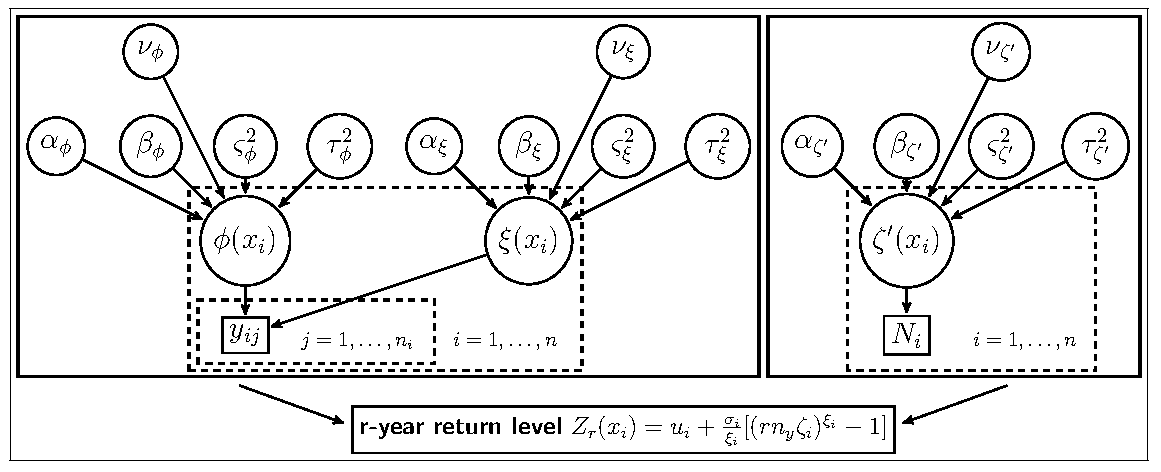
\includegraphics[scale = 0.8]{DAG2.pdf}

\section{Notation}

\begin{itemize}
\item $x_i$ Multivariate (bivariate or tri-variate) location values for location $i$, $i = 1,\ldots, n$. Write the matrix of all locations as just $x$
\item $y_{ij}$ Excess $j$ for observation $i$, $j = 1,\ldots,n_i$ where $n_i$ is the number of excesses at location $i$
\item $\sigma(x_i)$ Scale parameter for location $x_i$
\item $\phi(x_i) = \log(\sigma(x_i))$ The re-parameterised scale parameter
\item $\xi(x_i)$ Shape parameter for location $x_i$
\item $z_k$ Sub-grid locations $k = 1, \ldots, m$. Together written as $z$
\item $A, B$ Projection matrices of dimension $n \times m$
\item $\tilde{\phi}, \tilde{\xi}$ Gaussian processes of $\phi$ and $\xi$ defined on sub-grid $z$
\item $\mu_\phi(z), \mu_\xi(z)$ Means for the Gaussian processes
\item $\Sigma, \Psi$ Auto-covariance matrices for the Gaussian processes
\item $\tau^2_\phi, \tau^2_\xi$ Nugget standard deviation parameters
\item $\alpha_\phi, \alpha_\xi$ vectors of coefficients including intercept and slope parameters for Gaussian process means
\item $X_\phi, X_\xi, Z_\sigma, Z_\xi$ Matrices of covariates (including column for intercept term) on the $x$ grid and the $z$ sub-grid
\item $\nu_\phi, \nu_\xi$ Matern smoothness parameters
\item $\beta_\phi, \beta_\xi$ Matern length scale matrices
\item $\varsigma^2_\phi, \varsigma^2_\xi$ Variance parameters for Gaussian process
\end{itemize}

\section{Model outline} \label{outline}

In hierarchical notation:
\begin{align*}
y_{ij} &\sim GPD(\sigma(x_i), \xi(x_i)) \\
\log (\sigma (x)) = \phi(x) &= A(x, z) \Sigma^{-1}(z,z) \tilde{\phi}(z) \\
\xi (x) &= B(x, z) \Psi^{-1}(z,z) \tilde{\xi}(z) \\
A(x_i, z_k) &= \varsigma_\phi^2 \frac{2^{1-\nu_\phi}}{\Gamma(\nu_\phi)}\Bigg(\sqrt{2\nu_\phi}\frac{\|x_i - z_k\|}{\beta_\phi}\Bigg)^{\nu_\phi} K_{\nu_\phi}\Bigg(\sqrt{2\nu_\phi}\frac{\|x_i - z_k\|}{\beta_\phi}\Bigg)\\
B(x_i, z_k) &= \varsigma_\xi^2 \frac{2^{1-\nu_\xi}}{\Gamma(\nu_\xi)}\Bigg(\sqrt{2\nu_\xi}\frac{\|x_i - z_k\|}{\beta_\xi}\Bigg)^{\nu_\xi} K_{\nu_\xi}\Bigg(\sqrt{2\nu_\xi}\frac{\|x_i - z_k\|}{\beta_\xi}\Bigg)\\
\tilde{\phi} &\sim MVN_m(\mu_\phi(z), \tau_\phi^2 I_m + \Sigma(z, z))\\
\tilde{\xi} &\sim MVN_m(\mu_\xi(z), \tau_\xi^2 I_m + \Psi(z, z))\\
\mu_\phi (z) &= Z_\phi \alpha_\phi \\
\mu_\xi (z) &= Z_\xi \alpha_\xi \\
\mu_\phi(x) &= X_\phi \alpha_\phi \\
\mu_\xi(x) &= X_\xi \alpha_\xi \\
\Sigma(z_k, z_l) &= \varsigma_\phi^2 \frac{2^{1-\nu_\phi}}{\Gamma(\nu_\phi)}\Bigg(\sqrt{2\nu_\phi}\frac{\|z_k - z_l\|}{\beta_\phi}\Bigg)^{\nu_\phi} K_{\nu_\phi}\Bigg(\sqrt{2\nu_\phi}\frac{\|z_k - z_l\|}{\beta_\phi}\Bigg)\\
\Psi(z_k, z_l) &= \varsigma_\xi^2 \frac{2^{1-\nu_\xi}}{\Gamma(\nu_\xi)}\Bigg(\sqrt{2\nu_\xi}\frac{\|z_k - z_l\|}{\beta_\xi}\Bigg)^{\nu_\xi} K_{\nu_\xi}\Bigg(\sqrt{2\nu_\xi}\frac{\|z_k - z_l\|}{\beta_\xi}\Bigg)
\end{align*}

Hyper-parameter prior distributions (subject to change):
\begin{align*}
\log(\varsigma^2_\phi), \log(\varsigma^2_\xi), \log(\tau^2_\phi), \log(\tau^2_\xi) &\sim N(0, 10) \\
\beta_\phi, \beta_\xi, \nu_\phi, \nu_\xi &\sim DU(0.001, 0.01, 0.1, 1, 10, 100, 1000)\\
\alpha_\phi &\sim MVN(\vec{\eta}_\phi, H_\phi)\\
\alpha_\xi &\sim MVN(\vec{\eta}_\xi, H_\xi)\\
\end{align*}
To begin, $\vec{\eta}_\phi$ and $\vec{\eta}_\xi$ are vectors of the appropriate length with all entries equal to 0. $H_\phi$ and $H_\xi$ are the relevant covariance matrices - to begin, these are diagonal matrices with 10 on the diagonal. The code is designed to allow the relationship between the coefficients to be modelled (if desired) by adjusting this covariance matrix.

\section{Posterior distribution}

The full posterior distribution is:
\begin{align*}
p(\alpha_\phi, \alpha_\xi, \beta_\phi, \beta_\xi, \varsigma^2_\phi, \varsigma^2_\xi, \tau^2_\phi, \tau^2_\xi, \nu_\phi, \nu_\xi, \tilde{\phi}, \tilde{\xi} | y, x, z, X_\phi, X_\xi, Z_\phi, Z_\xi) \propto &\left[ \prod_{i=1}^n \prod_{j=1}^{n_i} p(y_{ij} | \sigma(x_i)=\exp(\phi(x_i)), \xi(x_i)) \right]  \times \\
& p(\tilde{\phi}(x) | \mu_\phi, \tau^2_\phi, \Sigma) p(\tilde{\xi}(x) | \mu_\xi, \tau^2_\xi, \Psi) \times \\
& p(\alpha_\phi) p(\alpha_\xi) p(\beta_\phi) p(\beta_\xi) p(\nu_\phi) p(\nu_\xi) \times \\
& p(\tau^2_\phi) p(\tau^2_\xi) p(\varsigma^2_\phi) p(\varsigma^2_\xi)
\end{align*}

\section{Conditional posterior distributions: Layer 1}

Updating the first layer of the DAG - that is, parameters $\tilde{\phi} = \log(\tilde{\sigma})$ and $\tilde{\xi}$. The conditional posterior distribution of $\tilde{\phi}$ is given by:

\begin{align*}
\pi(\tilde{\phi} | y, x, z, X_\phi, X_\xi, Z_\phi, Z_\xi, & \alpha_\phi, \alpha_\xi, \beta_\phi, \beta_\xi, \varsigma^2_\phi, \varsigma^2_\xi, \tau^2_\phi, \tau^2_\xi, \nu_\phi, \nu_\xi, \tilde{\xi}) \propto \\
& p(y | \tilde{\phi}, x, z, X_\phi, X_\xi, Z_\phi, Z_\xi, \alpha_\phi, \alpha_\xi, \beta_\phi, \beta_\xi, \varsigma^2_\phi, \varsigma^2_\xi, \tau^2_\phi, \tau^2_\xi, \nu_\phi, \nu_\xi, \tilde{\xi}) \times \\
& p(\tilde{\phi} | x, z, X_\phi, X_\xi, Z_\phi, Z_\xi, \alpha_\phi, \alpha_\xi, \beta_\phi, \beta_\xi, \varsigma^2_\phi, \varsigma^2_\xi, \tau^2_\phi, \tau^2_\xi, \nu_\phi, \nu_\xi, \tilde{\xi}) \\
\propto & p(y | \sigma, \xi)  p(\tilde{\phi} | \mu_\phi, \tau^2_\phi, \Sigma)
\end{align*}

That is, the conditional posterior of $\tilde{\phi}$ is proportional to the product of the likelihood of the data $y$ given $\tilde{\phi}$ and all other parameters, and the prior probability density of $\tilde{\phi}$ given all of the other parameters. In the final line, most parameters have dropped out from the right-hand side, as the densities are independent of
these, given the remaining terms (see the DAG for this). Of the remaining terms $\sigma, \xi, \mu_\phi$ and $\Sigma$ are all deterministic given the other parameters. These will have been calculated using the formulae in section \ref{outline}. \\

In briefer notation (to be used from now on):

\begin{align*}
\pi(\tilde{\phi} | \dots ) \propto & p(y | \phi, \xi)  p(\tilde{\phi} | \mu_\phi, \tau^2_\phi, \Sigma) \\
= & \left[ \prod_{i=1}^n \prod_{j=1}^{n_i} p(y_{ij} | \sigma(x_i), \xi(x_i)) \right] p(\tilde{\phi} | \mu_\phi, \tau^2_\phi, \Sigma) \\
= & \left[ \prod_{i=1}^n \prod_{j=1}^{n_i} \frac{1}{\sigma(x_i)} \bigg( 1 + \xi(x_i) \frac{y_{ij}}{\sigma(x_i)} \bigg)^{-(\sfrac{1}{\xi(x_i)} + 1)} \right] \times \\
& \frac{1}{\sqrt{\det(2 \pi (\Sigma + \tau^2_\phi I_m))}} e^{-\frac{1}{2} (\tilde{\phi} - \mu_\phi)' (\Sigma + \tau^2_\phi I_m)^{-1} (\tilde{\phi} - \mu_\phi) }
\end{align*}

Similarly:

\begin{align*}
\pi(\tilde{\xi} | \dots ) \propto & p(y | \phi, \xi)  p(\tilde{\xi} | \mu_\xi, \tau^2_\xi, \Psi) \\
= & \left[ \prod_{i=1}^n \prod_{j=1}^{n_i} p(y_{ij} | \sigma(x_i), \xi(x_i)) \right] p(\tilde{\xi} | \mu_\xi, \tau^2_\xi, \Psi) \\
= & \left[ \prod_{i=1}^n \prod_{j=1}^{n_i} \frac{1}{\sigma(x_i)} \bigg( 1 + \xi(x_i) \frac{y_{ij}}{\sigma(x_i)} \bigg)^{-(\sfrac{1}{\xi(x_i)} + 1)} \right] \times \\
& \frac{1}{\sqrt{\det(2 \pi (\Psi + \tau^2_\xi I_m))}} e^{-\frac{1}{2} (\tilde{\xi} - \mu_\xi)' (\Psi + \tau^2_\xi I_m)^{-1} (\tilde{\xi} - \mu_\xi) }
\end{align*}

\subsection{Metropolis-Hastings Markov chain Monte Carlo sampling}

In order to sample from these conditional posterior distributions, we use the Metropolis-Hastings Markov chain Monte Carlo (MCMC) algorithm. New samples are accepted or rejected at random according to the algorithm outlined below. \\

A new value of $\tilde{\phi_i}$ is suggested: $\tilde{\phi_i}'$. The new vector $\phi'$ is then calculated using the projection formula. \\

Though $\tilde{\phi}'$ differs from $\tilde{\phi}$ in just one location $i$, $\phi$ and $\phi'$ can be different from each other in many locations $i$ due to this projection. \\

Suggested updates are drawn from a Normal distribution centred on the old value and with a variance of a manually set tuning parameter used to control the size of the proposed steps. \\

We calculate:

\begin{align*}
\rho(\tilde{\phi_i}, \tilde{\phi'_i}) = \min \bigg (1, \frac{\pi(\tilde{\phi'} | \dots ) q_t(\tilde{\phi'_i} \to \tilde{\phi_i})}{ \pi(\tilde{\phi} | \dots ) q_t(\tilde{\phi_i} \to \tilde{\phi'_i}) } \bigg)
\end{align*}

where $\pi(\tilde{\phi} | \dots)$ is as defined above, and $q_t(a \to b)$ is the transition probability of proposing value $b$ given value $a$. Since updates are proposed using a Normal distribution, these transition probabilites above and below the line will always cancel, so the above simplifies to:

\begin{align*}
\rho(\tilde{\phi_i}, \tilde{\phi'_i}) = \min \bigg (1, \frac{\pi(\tilde{\phi'} | \dots ) }{ \pi(\tilde{\phi} | \dots ) } \bigg)
\end{align*}

Following this calculation, we always accept proposed value $\tilde{\phi'_i}$ when $\rho(\tilde{\phi_i}, \tilde{\phi'_i})$ is bigger than 1 and we reject accordingly when the ratio is smaller than 1 by simulating a random variable $u \sim U[0, 1]$ and accepting proposed value $\tilde{\phi'_i}$ when $u\leq \rho(\tilde{\phi_i}, \tilde{\phi'_i})$. \\

Evaluating $\rho(\tilde{\phi_i}, \tilde{\phi'_i})$ typically involves products and quotients of many terms which may be close to 0. In order to work with something far more stable, we use the property that $x = \exp(\log(x))$. \\ 

Following this observation we need to evaluate:

\begin{align*}
\exp \bigg( & \log \bigg (\frac{\pi(\tilde{\phi'} | \dots ) }{ \pi(\tilde{\phi} | \dots ) } \bigg) \bigg) \\
= \exp \big[ & \log(\pi(\tilde{\phi'} | \dots )) - \log(\pi(\tilde{\phi} | \dots )) \big] \\
= \exp \Big[ & \log \Big( \Big[ \prod_{i=1}^n \prod_{j=1}^{n_i} p(y_{ij} | \sigma'(x_i), \xi(x_i)) \Big] p(\tilde{\phi'} | \mu_\phi, \tau^2_\phi, \Sigma) \Big) - \\
& \log \Big( \Big[ \prod_{i=1}^n \prod_{j=1}^{n_i} p(y_{ij} | \sigma(x_i), \xi(x_i)) \Big] p(\tilde{\phi} | \mu_\phi, \tau^2_\phi, \Sigma) \Big) \Big]
\end{align*}

Filling in the specific distribution from above, this becomes:

\begin{align*}
 \exp \Bigg[ \log & \Big( \Big[ \prod_{i=1}^n \prod_{j=1}^{n_i} \frac{1}{\sigma'(x_i)} \bigg( 1 + \xi(x_i) \frac{y_{ij}}{\sigma'(x_i)} \bigg)^{-(\sfrac{1}{\xi(x_i)} + 1)} \Big] \times \\
& \frac{1}{\sqrt{\det(2 \pi (\Sigma + \tau^2_\phi I_m))}} e^{-\frac{1}{2} (\tilde{\phi'} - \mu_\phi)' (\Sigma + \tau^2_\phi I_m)^{-1} (\tilde{\phi'} - \mu_\phi) } \Big) \\
- \log & \Big( \Big[ \prod_{i=1}^n \prod_{j=1}^{n_i} \frac{1}{\sigma(x_i)} \bigg( 1 + \xi(x_i) \frac{y_{ij}}{\sigma(x_i)} \bigg)^{-(\sfrac{1}{\xi(x_i)} + 1)} \Big] \times \\
& \frac{1}{\sqrt{\det(2 \pi (\Sigma + \tau^2_\phi I_m))}} e^{-\frac{1}{2} (\tilde{\phi} - \mu_\phi)' (\Sigma + \tau^2_\phi I_m)^{-1} (\tilde{\phi} - \mu_\phi) } \Big) \Bigg] \\
= \exp \Bigg[ \sum_{i=1}^n \sum_{j=1}^{n_i} \log & \Big( \Big[ \frac{1}{\sigma'(x_i)} \bigg( 1 + \xi(x_i) \frac{y_{ij}}{\sigma'(x_i)} \bigg)^{-(\sfrac{1}{\xi(x_i)} + 1)} \Big] \Big) + \\
& \log \Bigg( \frac{1}{\sqrt{\det(2 \pi (\Sigma + \tau^2_\phi I_m))}} \Bigg) -\frac{1}{2} (\tilde{\phi'} - \mu_\phi)' (\Sigma + \tau^2_\phi I_m)^{-1} (\tilde{\phi'} - \mu_\phi) \\
- \sum_{i=1}^n \sum_{j=1}^{n_i} \log & \Big( \Big[  \frac{1}{\sigma(x_i)} \bigg( 1 + \xi(x_i) \frac{y_{ij}}{\sigma(x_i)} \bigg)^{-(\sfrac{1}{\xi(x_i)} + 1)} \Big] \Big) - \\
& \log \Bigg( \frac{1}{\sqrt{\det(2 \pi (\Sigma + \tau^2_\phi I_m))}} \Bigg) +\frac{1}{2} (\tilde{\phi} - \mu_\phi)' (\Sigma + \tau^2_\phi I_m)^{-1} (\tilde{\phi} - \mu_\phi) \Bigg] \\
= \exp \Bigg[ \sum_{i=1}^n \sum_{j=1}^{n_i} \log & \Big( \Big[ \frac{1}{\sigma'(x_i)} \bigg( 1 + \xi(x_i) \frac{y_{ij}}{\sigma'(x_i)} \bigg)^{-(\sfrac{1}{\xi(x_i)} + 1)} \Big] \Big) -\frac{1}{2} (\tilde{\phi'} - \mu_\phi)' (\Sigma + \tau^2_\phi I_m)^{-1} (\tilde{\phi'} - \mu_\phi) \\
- \sum_{i=1}^n \sum_{j=1}^{n_i} \log & \Big( \Big[  \frac{1}{\sigma(x_i)} \bigg( 1 + \xi(x_i) \frac{y_{ij}}{\sigma(x_i)} \bigg)^{-(\sfrac{1}{\xi(x_i)} + 1)} \Big] \Big) +\frac{1}{2} (\tilde{\phi} - \mu_\phi)' (\Sigma + \tau^2_\phi I_m)^{-1} (\tilde{\phi} - \mu_\phi) \Bigg]
\end{align*}

The common term in both numerator and denominator above dropped out as it will be equal in both (it has no dependence on $\tilde{\phi}$). \\

The GPD can clearly be simplified further using the properties of logs. Just taking one of the functions on its own for clarity:

\begin{align*}
\sum_{i=1}^n \sum_{j=1}^{n_i} \log & \Bigg( \Bigg[ \frac{1}{\sigma'(x_i)} \bigg( 1 + \xi(x_i) \frac{y_{ij}}{\sigma'(x_i)} \bigg)^{-(\sfrac{1}{\xi(x_i)} + 1)} \Bigg] \Bigg) = \\
\sum_{i=1}^n \sum_{j=1}^{n_i} \Bigg[ \log & \Big( \frac{1}{\sigma'(x_i)} \Big) + \log \bigg( 1 + \xi(x_i) \frac{y_{ij}}{\sigma'(x_i)} \bigg)^{-(\sfrac{1}{\xi(x_i)} + 1)} \Bigg] = \\
\sum_{i=1}^n \sum_{j=1}^{n_i} \Bigg[ - \log & (\sigma'(x_i)) - \bigg( \frac{1}{\xi(x_i)} + 1 \bigg) \log \bigg( 1 + \xi(x_i) \frac{y_{ij}}{\sigma'(x_i)} \bigg) \Bigg]
\end{align*}

Following this, the full term we need to evaluate in order to update $\tilde{\phi}$ is:

\begin{align}
= \exp \Bigg[ \sum_{i=1}^n \sum_{j=1}^{n_i} & \bigg[ - \log (\sigma'(x_i)) - \bigg( \frac{1}{\xi(x_i)} + 1 \bigg) \log \bigg( 1 + \xi(x_i) \frac{y_{ij}}{\sigma'(x_i)} \bigg) \bigg] -\frac{1}{2} (\tilde{\phi'} - \mu_\phi)' (\Sigma + \tau^2_\phi I_m)^{-1} (\tilde{\phi'} - \mu_\phi) \nonumber \\
- \sum_{i=1}^n \sum_{j=1}^{n_i} & \bigg[ - \log (\sigma(x_i)) - \bigg( \frac{1}{\xi(x_i)} + 1 \bigg) \log \bigg( 1 + \xi(x_i) \frac{y_{ij}}{\sigma(x_i)} \bigg) \bigg] +\frac{1}{2} (\tilde{\phi} - \mu_\phi)' (\Sigma + \tau^2_\phi I_m)^{-1} (\tilde{\phi} - \mu_\phi) \Bigg] \label{eq:1a}
\end{align}

Similar reasoning leads to the update for $\tilde{\xi}$. We need to evaluate:

\begin{align*}
\rho(\tilde{\xi_i}, \tilde{\xi'_i}) = \min \bigg (1, \frac{\pi(\tilde{\xi'} | \dots ) q_t(\tilde{\xi'_i} \to \tilde{\xi_i})}{ \pi(\tilde{\xi} | \dots ) q_t(\tilde{\xi_i} \to \tilde{\xi'_i}) } \bigg)
\end{align*}

The full term we need to evaluate is:

\begin{align}
= \exp \Bigg[ \sum_{i=1}^n \sum_{j=1}^{n_i} & \bigg[ - \log (\sigma(x_i)) - \bigg( \frac{1}{\xi'(x_i)} + 1 \bigg) \log \bigg( 1 + \xi'(x_i) \frac{y_{ij}}{\sigma(x_i)} \bigg) \bigg] -\frac{1}{2} (\tilde{\xi'} - \mu_\xi)' (\Psi + \tau^2_\xi I_m)^{-1} (\tilde{\xi'} - \mu_\xi) \nonumber \\
- \sum_{i=1}^n \sum_{j=1}^{n_i} & \bigg[ - \log (\sigma(x_i)) - \bigg( \frac{1}{\xi(x_i)} + 1 \bigg) \log \bigg( 1 + \xi(x_i) \frac{y_{ij}}{\sigma(x_i)} \bigg) \bigg] +\frac{1}{2} (\tilde{\xi} - \mu_\xi)' (\Psi + \tau^2_\xi I_m)^{-1} (\tilde{\xi} - \mu_\xi) \Bigg] \label{eq:1b}
\end{align}


\section{Conditional posterior distributions: Layer 2}

\subsection{$\alpha$}

Updating the second layer of the DAG - that is, all hyper-parameters - starting with $\alpha_\phi$:

\begin{align*}
\pi(\alpha_\phi | y, \dots ) \propto & p(y | \alpha_\phi, \dots ) p(\alpha_\phi | \dots) \\
\propto & p(y | \sigma, \xi)  p(\tilde{\phi} | \mu_\phi, \tau^2_\phi, \Sigma) p(\alpha_\phi) \\
\propto & p(\tilde{\phi} | \mu_\phi, \tau^2_\phi, \Sigma) p(\alpha_\phi)
\end{align*}

Essentially the GPD component is independent of $\alpha_\phi$ once the other parameters are known, and so can be absorbed into the constant of proportionality. What we're left with is the $MVN$ piece (since $\alpha_\phi$ features in the calculation of $\mu_\phi$) and the prior on $\alpha_\phi$. \\

Then we have:

\begin{align*}
\pi(\alpha_\phi | \dots ) \propto & p(\tilde{\phi} | \mu_\phi, \tau^2_\phi, \Sigma) p(\alpha_\phi) \\
\propto & \frac{1}{\sqrt{\det(2 \pi (\Sigma + \tau^2_\phi I_m))}} e^{-\frac{1}{2} (\tilde{\phi} - \mu_\phi)' (\Sigma + \tau^2_\phi I_m)^{-1} (\tilde{\phi} - \mu_\phi) } \times \\
& \frac{1}{\sqrt{\det(2 \pi H_\phi)}} e^{-\frac{1}{2} (\alpha_\phi - \eta_\phi)' H_\phi^{-1} (\alpha_\phi - \eta_\phi) }
\end{align*}

where $H_\phi$ is the covariance matrix for the prior distribution of $\alpha_\phi$ and $\eta_\phi$ is the prior mean.

Similarly:

\begin{align*}
\pi(\alpha_\xi | \dots ) \propto & p(\tilde{\xi} | \mu_\xi, \tau^2_\xi, \Psi) p(\alpha_\xi) \\
\propto & \frac{1}{\sqrt{\det(2 \pi (\Psi + \tau^2_\xi I_m))}} e^{-\frac{1}{2} (\tilde{\xi} - \mu_\xi)' (\Psi + \tau^2_\xi I_m)^{-1} (\tilde{\xi} - \mu_\xi) } \times \\
& \frac{1}{\sqrt{\det(2 \pi H_\xi)}} e^{-\frac{1}{2} (\alpha_\xi - \eta_\xi)' H_\xi^{-1} (\alpha_\xi - \eta_\xi) }
\end{align*}

where $H_\xi$ is the covariance matrix for the prior distribution of $\alpha_\xi$ and $\eta_\xi$ is the prior mean. \\

As before, updates are suggested for alpha element-wise: $\alpha_{\phi,k} \to \alpha'_{\phi,k}$. The ratio $\rho(\alpha_{\phi,k}, \alpha'_{\phi,k})$ is then calculated. Similar manipulations to those used in the previous section lead to the following calculation needed to update $\alpha_\phi$:

\begin{align}
\exp \Big[ - \frac{1}{2} & \log(\det(2 \pi (\Sigma + \tau^2_\phi I_m))) -\frac{1}{2} (\tilde{\phi} - \mu_\phi)' (\Sigma + \tau^2_\phi I_m)^{-1} (\tilde{\phi} - \mu_\phi) \nonumber \\
& - \frac{1}{2} \log(\det(2 \pi H_\phi)) -\frac{1}{2} (\alpha'_\phi - \eta_\phi)' H_\phi^{-1} (\alpha'_\phi - \eta_\phi) ) \nonumber \\
& + \frac{1}{2} \log(\det(2 \pi (\Sigma + \tau^2_\phi I_m))) + \frac{1}{2} (\tilde{\phi} - \mu_\phi)' (\Sigma + \tau^2_\phi I_m)^{-1} (\tilde{\phi} - \mu_\phi) \nonumber \\
& + \frac{1}{2} \log(\det(2 \pi H_\phi)) + \frac{1}{2} (\alpha_\phi - \eta_\phi)' H_\phi^{-1} (\alpha_\phi - \eta_\phi) )
\Big] = \nonumber \\
\exp \Big[ -\frac{1}{2} & (\tilde{\phi} - \mu_\phi)' (\Sigma + \tau^2_\phi I_m)^{-1} (\tilde{\phi} - \mu_\phi) -\frac{1}{2} (\alpha'_\phi - \eta_\phi)' H_\xi^{-1} (\alpha'_\phi - \eta_\phi) ) \nonumber \\
& + \frac{1}{2} (\tilde{\phi} - \mu_\phi)' (\Sigma + \tau^2_\phi I_m)^{-1} (\tilde{\phi} - \mu_\phi) + \frac{1}{2} (\alpha_\phi - \eta_\phi)' H_\phi^{-1} (\alpha_\phi - \eta_\phi) )
\Big] \label{eq:2a1}
\end{align}

And for $\alpha_\xi$:

\begin{align}
\exp \Big[ -\frac{1}{2} & (\tilde{\xi} - \mu_\xi)' (\Psi + \tau^2_\xi I_m)^{-1} (\tilde{\xi} - \mu_\xi) -\frac{1}{2} (\alpha'_\xi - \eta_\xi)' H_\xi^{-1} (\alpha'_\xi - \eta_\xi) ) \nonumber \\
& + \frac{1}{2} (\tilde{\xi} - \mu_\xi)' (\Psi + \tau^2_\xi I_m)^{-1} (\tilde{\xi} - \mu_\xi) + \frac{1}{2} (\alpha_\xi - \eta_\xi)' H_\xi^{-1} (\alpha_\xi - \eta_\xi) )
\Big] \label{eq:2a2}
\end{align}

Updates for the other hyper-parameters are very similar - though none feature the $MVN$ prior that $\alpha_\phi$ and $\alpha_\xi$ do, the part involving the log determinant can't be dropped from the $m$-dim $MVN$, since the matrix changes with any change in $\beta, \nu, \varsigma^2$ or $\tau^2$. The remaining hyper-parameters either have a discrete update (in which case the prior probability will be $\sfrac{1}{\#discrete.values}$ and will cancel above and below the line, or have a univariate Normal prior on them (or their log). \\

\subsection{$\beta$}

For $\beta_\phi$ we have:

\begin{align*}
\pi(\beta_\phi | \dots ) \propto & p(\tilde{\phi} | \mu_\phi, \tau^2_\phi, \Sigma) p(\beta_\phi)
\end{align*}

Since $\beta_\phi$ has a discrete prior, to update $\beta_\phi$ we need to evaluate:

\begin{align}
\exp \Big[ & - \frac{1}{2}  \log(\det(2 \pi (\Sigma' + \tau^2_\phi I_m))) -\frac{1}{2} (\tilde{\phi} - \mu_\phi)' (\Sigma' + \tau^2_\phi I_m)^{-1} (\tilde{\phi} - \mu_\phi) \nonumber \\
& + \frac{1}{2} \log(\det(2 \pi (\Sigma + \tau^2_\phi I_m))) + \frac{1}{2} (\tilde{\phi} - \mu_\phi)' (\Sigma + \tau^2_\phi I_m)^{-1} (\tilde{\phi} - \mu_\phi) \Big] \label{eq:2b1}
\end{align}

where $\Sigma'$ has been formed using $\beta'_\phi$, the new proposal value. \\

Then for $\beta_\xi$ we have:

\begin{align*}
\pi(\beta_\xi | \dots ) \propto & p(\tilde{\xi} | \mu_\xi, \tau^2_\xi, \Psi) p(\beta_\xi)
\end{align*}

To update $\beta_\xi$ we need to evaluate:

\begin{align}
\exp \Big[ & -\frac{1}{2} \log(\det(2 \pi (\Psi' + \tau^2_\xi I_m))) -\frac{1}{2} (\tilde{\xi} - \mu_\xi)' (\Psi' + \tau^2_\xi I_m)^{-1} (\tilde{\xi} - \mu_\xi) \nonumber \\
& + \frac{1}{2} \log(\det(2 \pi (\Psi + \tau^2_\xi I_m)))+ \frac{1}{2} (\tilde{\xi} - \mu_\xi)' (\Psi + \tau^2_\xi I_m)^{-1} (\tilde{\xi} - \mu_\xi) \Big] \label{eq:2b2}
\end{align}

where $\Psi'$ has been formed using $\beta'_\xi$, the new proposal value. \\

\subsection{$\nu$}

$\nu_\phi$ also has a discrete update and so will look identical to the update for $\beta_\phi$. It has conditional posterior distribution of:

\begin{align*}
\pi(\nu_\phi | \dots ) \propto & p(\tilde{\phi} | \mu_\phi, \tau^2_\phi, \Sigma) p(\nu_\phi)
\end{align*}

We need to evaluate:

\begin{align}
\exp \Big[ & - \frac{1}{2}  \log(\det(2 \pi (\Sigma' + \tau^2_\phi I_m))) -\frac{1}{2} (\tilde{\phi} - \mu_\phi)' (\Sigma' + \tau^2_\phi I_m)^{-1} (\tilde{\phi} - \mu_\phi) \nonumber \\
& + \frac{1}{2} \log(\det(2 \pi (\Sigma + \tau^2_\phi I_m))) + \frac{1}{2} (\tilde{\phi} - \mu_\phi)' (\Sigma + \tau^2_\phi I_m)^{-1} (\tilde{\phi} - \mu_\phi) \Big] \label{eq:2n1}
\end{align}

where $\Sigma'$ has been formed using $\nu'_\phi$, the new proposal value. \\

In order to update $\nu_\xi$ we have:

\begin{align*}
\pi(\nu_\xi | \dots ) \propto & p(\tilde{\xi} | \mu_\xi, \tau^2_\xi, \Psi) p(\nu_\xi)
\end{align*}

We therefore need to evaluate:

\begin{align}
\exp \Big[ & -\frac{1}{2} \log(\det(2 \pi (\Psi' + \tau^2_\xi I_m))) -\frac{1}{2} (\tilde{\xi} - \mu_\xi)' (\Psi' + \tau^2_\xi I_m)^{-1} (\tilde{\xi} - \mu_\xi) \nonumber \\
& + \frac{1}{2} \log(\det(2 \pi (\Psi + \tau^2_\xi I_m)))+ \frac{1}{2} (\tilde{\xi} - \mu_\xi)' (\Psi + \tau^2_\xi I_m)^{-1} (\tilde{\xi} - \mu_\xi) \Big] \label{eq:2n2}
\end{align}

where $\Psi'$ has been formed using $\nu'_\xi$, the new proposal value. \\

\subsection{$\varsigma^2$}

$\varsigma^2_\phi$ has a conditional posterior distribution of:

\begin{align*}
\pi(\varsigma^2_\phi | \dots ) \propto & p(\tilde{\phi} | \mu_\phi, \tau^2_\phi, \Sigma) p(\varsigma^2_\phi)
\end{align*}

The prior distribution of the log of $\varsigma^2_\phi$ is a univariate Normal. So to update $\varsigma^2_\phi$ we need to evaluate:

\begin{align}
\exp \Bigg[ & - \frac{1}{2}  \log(\det(2 \pi (\Sigma' + \tau^2_\phi I_m))) -\frac{1}{2}  (\tilde{\phi} - \mu_\phi)' (\Sigma' + \tau^2_\phi I_m)^{-1} (\tilde{\phi} - \mu_\phi) - \frac{(\log(\varsigma^{2'}_\phi) - m)^2}{2 s^2} \nonumber \\
& + \frac{1}{2}  \log(\det(2 \pi (\Sigma + \tau^2_\phi I_m))) + \frac{1}{2} (\tilde{\phi} - \mu_\phi)' (\Sigma + \tau^2_\phi I_m)^{-1} (\tilde{\phi} - \mu_\phi) + \frac{(\log(\varsigma^2_\phi) - m)^2}{2 s^2} \Bigg] \label{eq:2vs1}
\end{align}

where $\Sigma'$ has been formed using $\varsigma^{2'}_\phi$, the new proposal value, and $m$ and $s$ are the prior mean and standard deviation repectively. \\

$\varsigma^2_\xi$ has a conditional posterior distribution of:

\begin{align*}
\pi(\varsigma^2_\xi | \dots ) \propto & p(\tilde{\xi} | \mu_\xi, \tau^2_\xi, \Psi) p(\varsigma^2_\xi)
\end{align*}

To update $\varsigma^2_\xi$ we need to evaluate:

\begin{align}
\exp \Bigg[ & -\frac{1}{2} \log(\det(2 \pi (\Psi' + \tau^2_\xi I_m))) -\frac{1}{2}  (\tilde{\xi} - \mu_\xi)' (\Psi' + \tau^2_\xi I_m)^{-1} (\tilde{\xi} - \mu_\xi) - \frac{(\log(\varsigma^{2'}_\xi) - m)^2}{2 s^2} \nonumber \\
& +  \frac{1}{2} \log(\det(2 \pi (\Psi + \tau^2_\xi I_m))) + \frac{1}{2} (\tilde{\xi} - \mu_\xi)' (\Psi + \tau^2_\xi I_m)^{-1} (\tilde{\xi} - \mu_\xi) + \frac{(\log(\varsigma^2_\xi) - m)^2}{2 s^2} \Bigg] \label{eq:2vs2}
\end{align}

where $\Psi'$ has been formed using $\varsigma^{2'}_\xi$, the new proposal value, and $m$ and $s$ are the prior mean and standard deviation repectively. \\

\subsection{$\tau^2$}

$\tau^2_\phi$ has a conditional posterior distribution of:

\begin{align*}
\pi(\tau^2_\phi | \dots ) \propto & p(\tilde{\phi} | \mu_\phi, \tau^2_\phi, \Sigma) p(\tau^2_\phi)
\end{align*}

The prior distribution of the log of $\tau^2_\phi$ is a univariate Normal. So to update $\tau^2_\phi$ we need to evaluate:

\begin{align}
\exp \Bigg[ & - \frac{1}{2}  \log(\det(2 \pi (\Sigma + \tau^{2'}_\phi I_m))) -\frac{1}{2}  (\tilde{\phi} - \mu_\phi)' (\Sigma + \tau^{2'}_\phi I_m)^{-1} (\tilde{\phi} - \mu_\phi) - \frac{(\log(\tau^{2'}_\phi) - m)^2}{2 s^2} \nonumber \\
& +  \frac{1}{2}  \log(\det(2 \pi (\Sigma + \tau^2_\phi I_m))) +  \frac{1}{2} (\tilde{\phi} - \mu_\phi)' (\Sigma + \tau^2_\phi I_m)^{-1} (\tilde{\phi} - \mu_\phi) + \frac{(\log(\tau^2_\phi) - m)^2}{2 s^2} \Bigg] \label{eq:2t1}
\end{align}

where $m$ and $s$ are the prior mean and standard deviation repectively. \\

$\tau^2_\xi$ has a conditional posterior distribution of:

\begin{align*}
\pi(\tau^2_\xi | \dots ) \propto & p(\tilde{\xi} | \mu_\xi, \tau^2_\xi, \Psi) p(\tau^2_\xi)
\end{align*}

To update $\tau^2_\xi$ we need to evaluate:

\begin{align}
\exp \Bigg[ & -\frac{1}{2} \log(\det(2 \pi (\Psi + \tau^{2'}_\xi I_m))) -\frac{1}{2}  (\tilde{\xi} - \mu_\xi)' (\Psi + \tau^{2'}_\xi I_m)^{-1} (\tilde{\xi} - \mu_\xi) - \frac{(\log(\tau^{2'}_\xi) - m)^2}{2 s^2} \nonumber \\
& + \frac{1}{2} \log(\det(2 \pi (\Psi + \tau^{2}_\xi I_m))) +  \frac{1}{2} (\tilde{\xi} - \mu_\xi)' (\Psi + \tau^2_\xi I_m)^{-1} (\tilde{\xi} - \mu_\xi) + \frac{(\log(\tau^2_\xi) - m)^2}{2 s^2} \Bigg] \label{eq:2t2}
\end{align}

where $m$ and $s$ are the prior mean and standard deviation repectively. \\


\end{document}
